
\begin{frame}{Experiments}
    \begin{itemize}
        \item Datasets
        \vspace{1em}
        \item Design of Experiments
        \vspace{1em}
        \item Results
    \end{itemize}
\end{frame}


\begin{frame}{Experiments: Datasets}
\begin{itemize}
    \item \textbf{No public real bank dataset found}. Confidential and private nature of bank data.
    \vspace{1em}
    \item \textbf{Synthetic bank dataset generation tool}: 
    \begin{itemize}
        \item[(i)] Bank database.
        \vspace{0.5em}
        \item[(ii)] Transactions stream.
    \end{itemize}
    \vspace{1em}
    \begin{itemize}
        \item[$\Rightarrow$] Customisable data generation.
        \vspace{0.5em}
        \item[$\Rightarrow$] Based on a previously developed synthetic bank database \emph{Wisabi Bank Dataset} (publicly available). Used as a reference for the geographical distribution of ATM locations and card/client transaction \emph{behavior}.
        \vspace{0.5em}
        \item[$\Rightarrow$] Left as a public available tool.\footnote{\url{https://github.com/FCanfran/ATM-DP/tree/main/gdb}}
    \end{itemize}    
\end{itemize}
\end{frame}

\begin{frame}{Experiments: Datasets}
\begin{itemize}
    \item \textbf{(i) Bank database generator}. \texttt{bankDataGenerator.py}: creates a dataset of $n$ ATMs and $m$ Cards.
    \vspace{0.4em}
    \item \textbf{(ii) Transaction stream generator}. \texttt{txGenerator.py}: parametrizable, with $\texttt{ratio} \in [0,1]$ of anomalous tx..
    \vspace{0.2em}
    \begin{itemize}
        \item 1. \emph{Regular} transactions: avoiding creation of fraud scenarios. Based on gathered customer \emph{behavior} from \emph{Wisabi DS}.
        \vspace{0.3em}
        \item 2. Injection of transactions that create anomalous scenarios: tailored injection depending on the ATM fraud considered.
    \end{itemize}
\end{itemize}
\begin{figure}
    \centering
    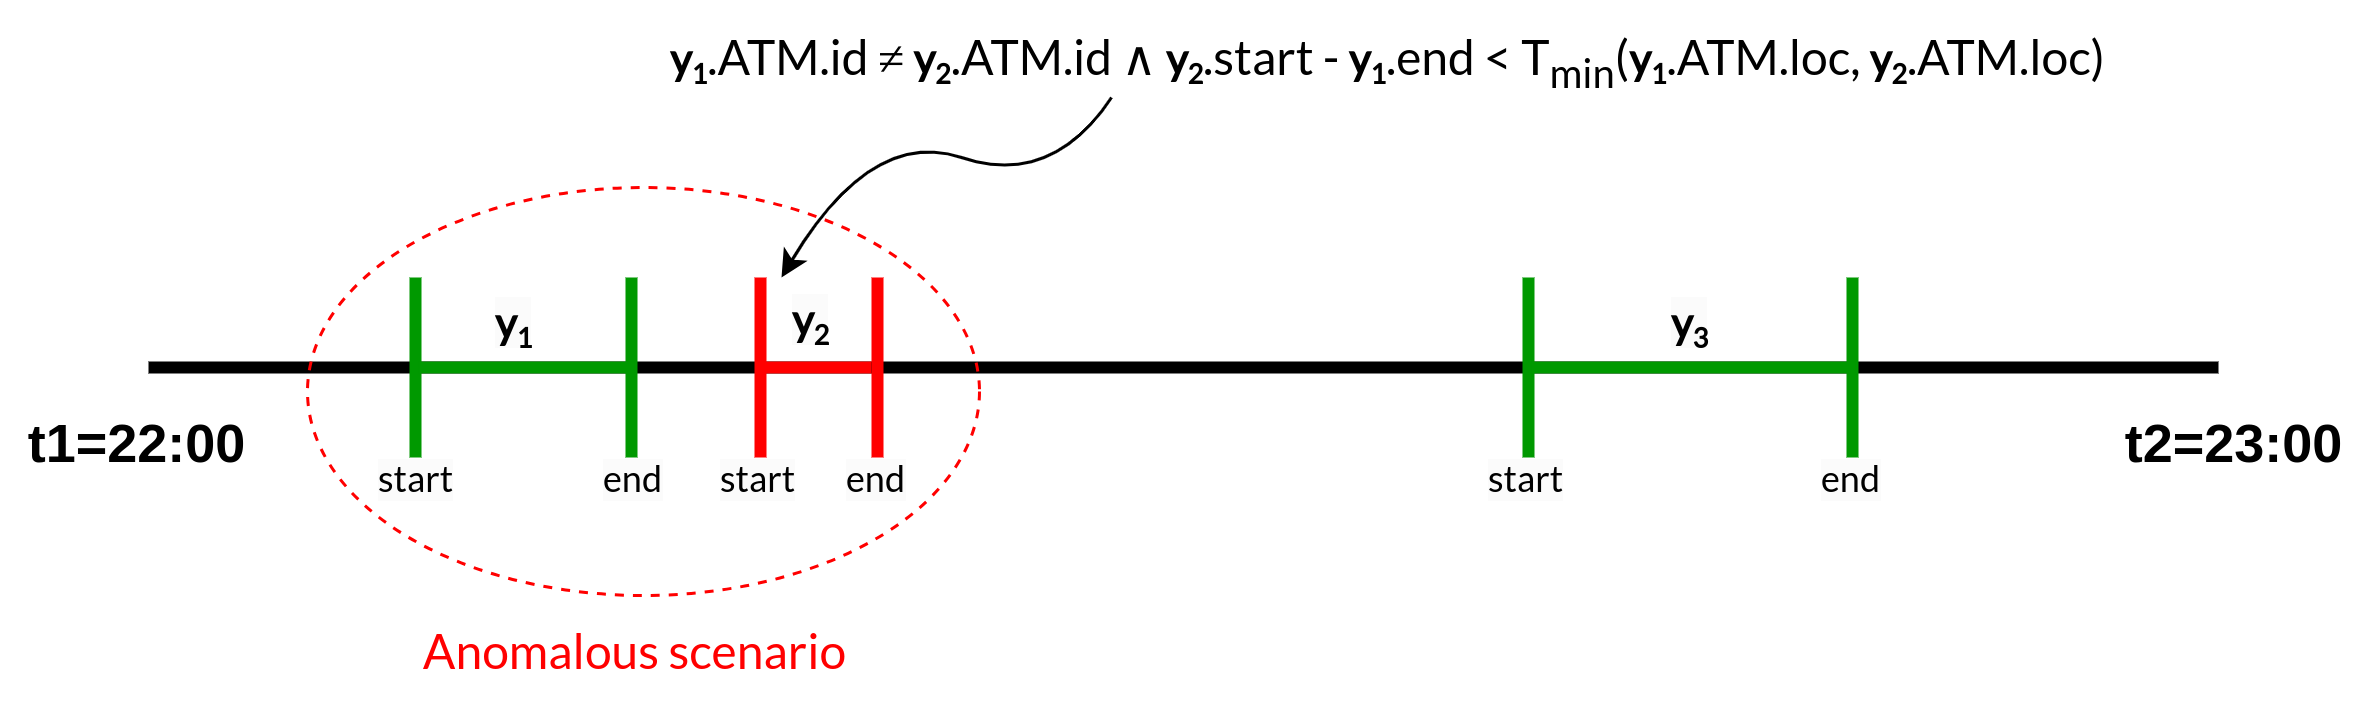
\includegraphics[width=\textwidth]{figures/tx-generation.png}
    \caption{Creation of anomalous scenario I - Card cloning}
\end{figure}
\end{frame}

\begin{comment}
\begin{frame}{Experiments: Datasets}

\begin{itemize}
    \item 1. Generation of \emph{regular} transactions: ensuring that do not create fraud scenarios. 
    \item 2. Injection of transactions that create anomalous scenarios: \textcolor{red}{taylored injection} depending on the ATM fraud considered.
\end{itemize}
\begin{figure}
    \centering
    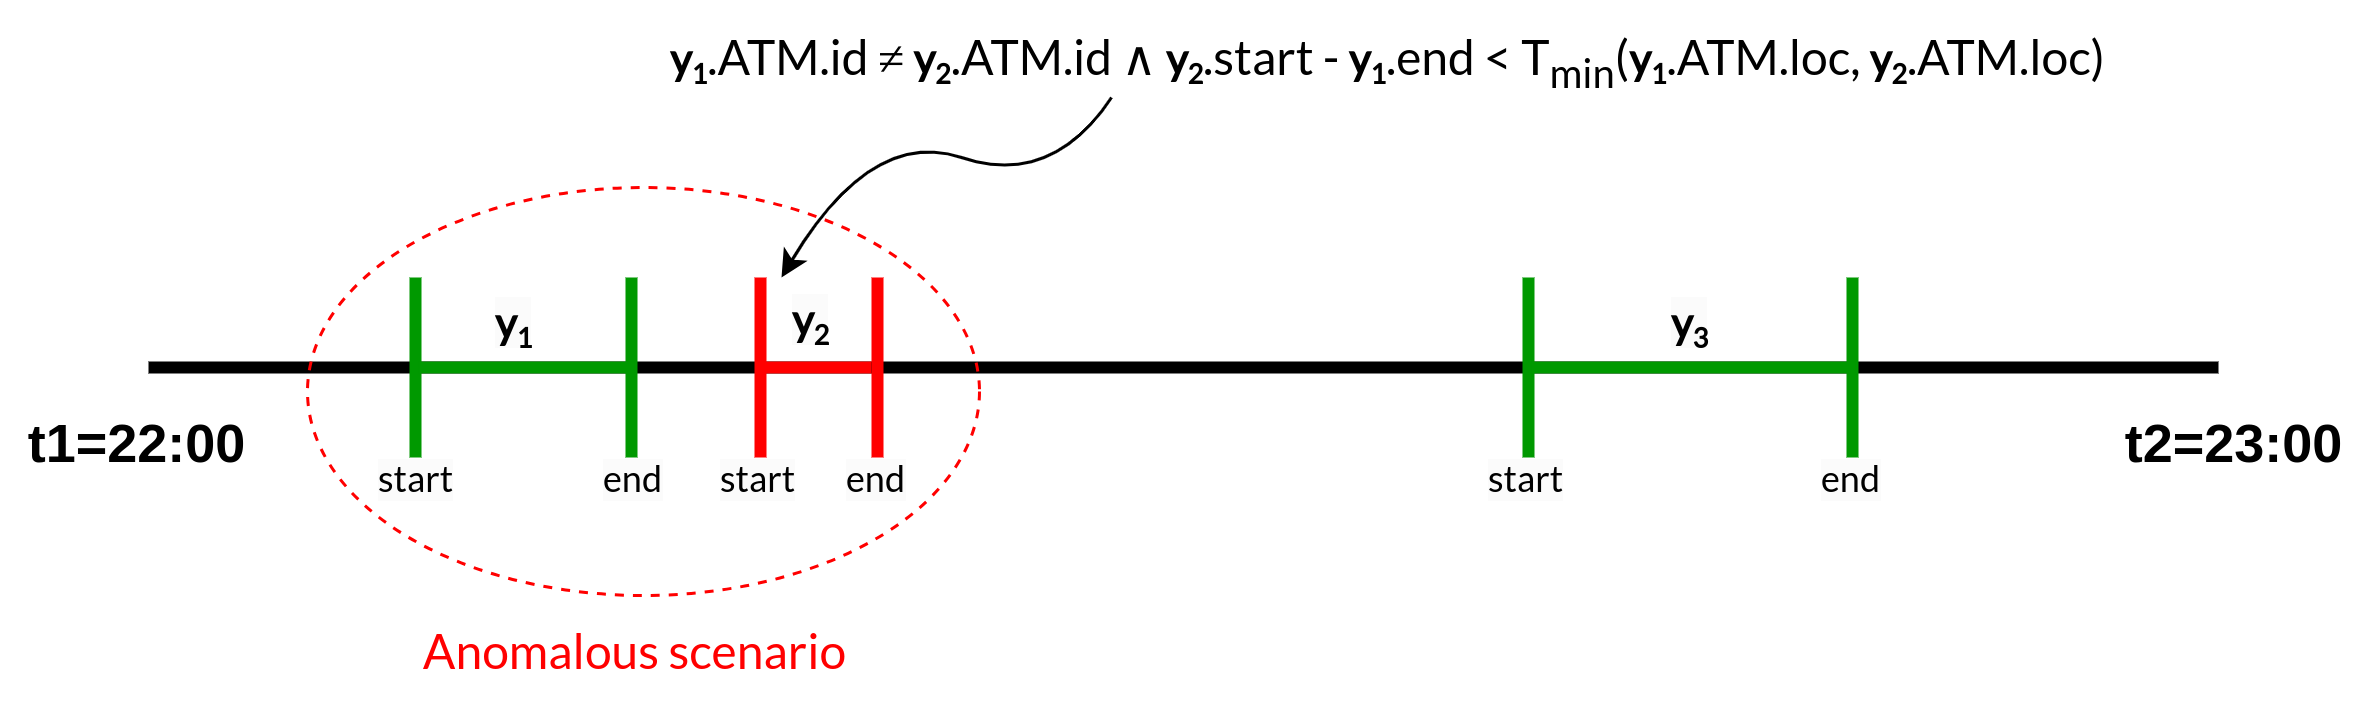
\includegraphics[width=\textwidth]{figures/tx-generation.png}
    \caption{Creation of anomalous scenario I - Card cloning}
\end{figure}
\end{frame}
\end{comment}

\begin{comment}
\begin{frame}{Experimental Design:: Anomalous scenarios (I)}
\begin{itemize}
    \item $\texttt{ratio} \in [0,1]$ s.t. $\texttt{ratio} * \texttt{num\_tx}$ is the number of anomalous scenarios created for a card in the considered time interval $[0,t]$.
    \item No overlapping of the transaction introduced $a$ with the regular ones $i, i+1$: $T_i + \Delta_i < T_a < T_a + \Delta_a < T_{i+1}$
\end{itemize}

\begin{figure}
    \centering
    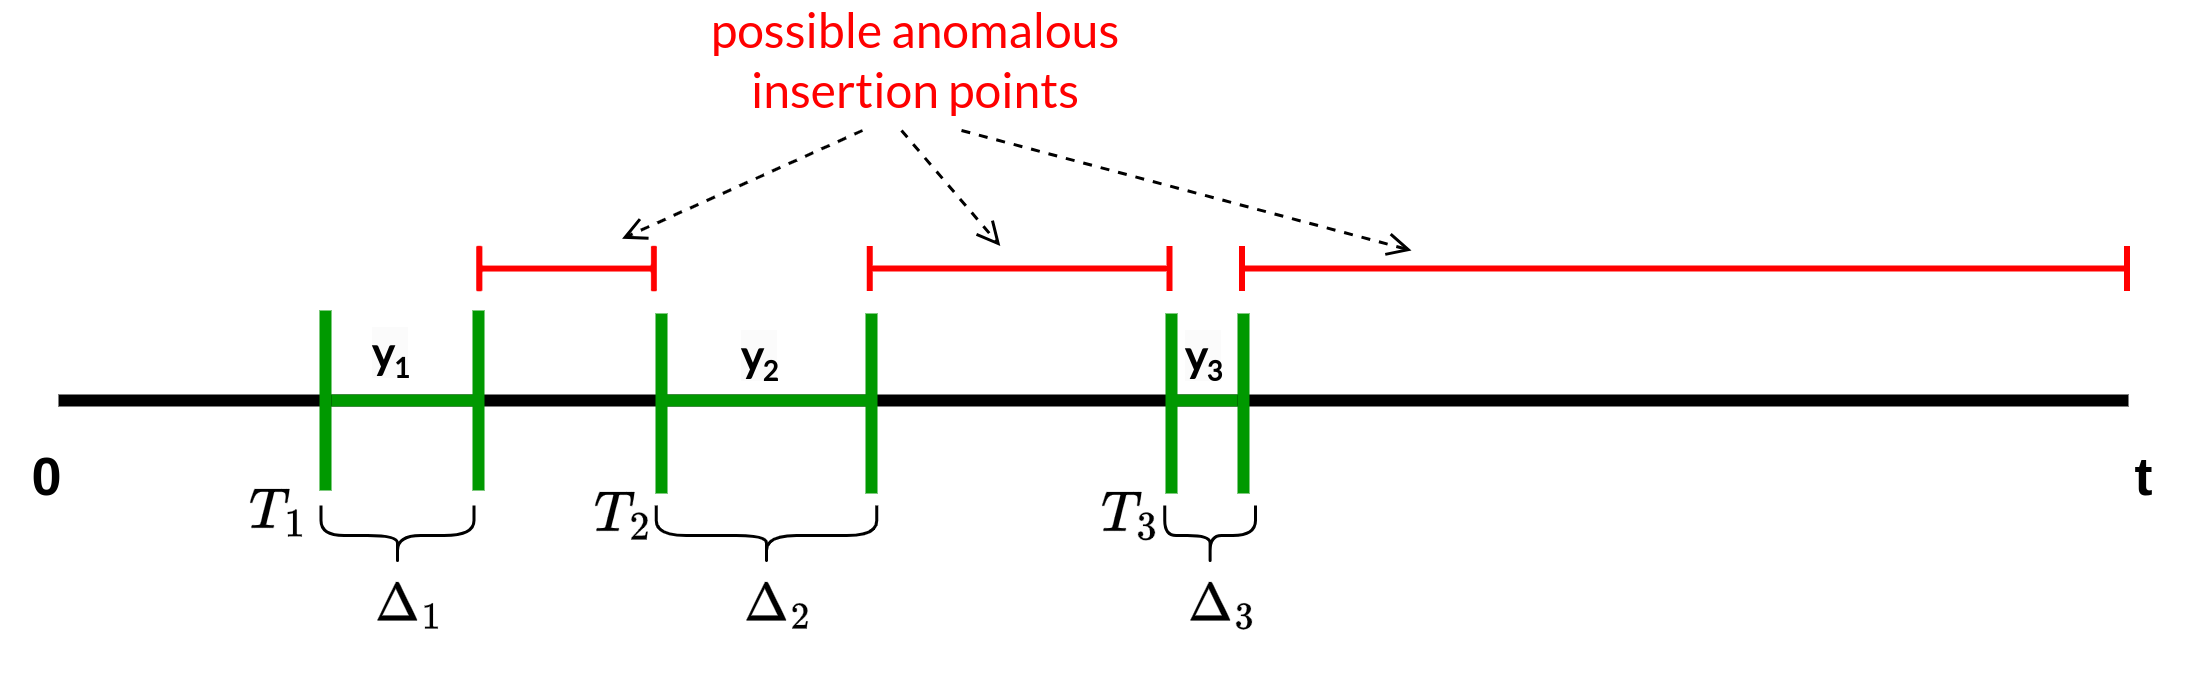
\includegraphics[width=\textwidth]{figures/tx-generation-anomalous-1.png}
\end{figure}
\end{frame}
\end{comment}

\begin{comment}
\begin{frame}{Experimental Design:: Interaction Generation}
Considerations:
\vspace{1em}
\begin{itemize}
    \item Particular ATM usage frequency
    \vspace{1em}
    \item ATM selection for the generated transactions of each card
    \vspace{1em}
    \item Distribution of the generated transactions on the decided considered time
    \vspace{0.5em}
\end{itemize}

\begin{itemize}
    \item 
    \begin{itemize}
        \item[$\circ$] ATM - Pre-selection of closed card ATM subset
        \item[$\circ$] Time - Uniform distribution
        \item[$\circ$] Time - Poisson process distribution
        \item[$\circ$] Random walks
        \item[$\circ$] ...
    \end{itemize}
    
\end{itemize}
\end{frame}
\end{comment}

\begin{comment}
% TODO: Select which one
\begin{frame}{Experimental Design:: Regular transactions}
Idea: For each card, generate a set of \emph{regular} transactions for a $d$ number of days (starting on a selected $start\_date$). 
%// ALTERNATIVE: for a selected window of time
\begin{itemize}
    \item Limiting the regular transactions of the client to $\texttt{Neighborhood}$.
    (ATM $\in \texttt{Neighborhood}$).
\end{itemize}

$$\texttt{Neighborhood} = \{\texttt{ATM}\ | \texttt{dist(ATM, residence\_loc)} \leq \texttt{max\_distance}\}$$

\begin{figure}
    \centering
    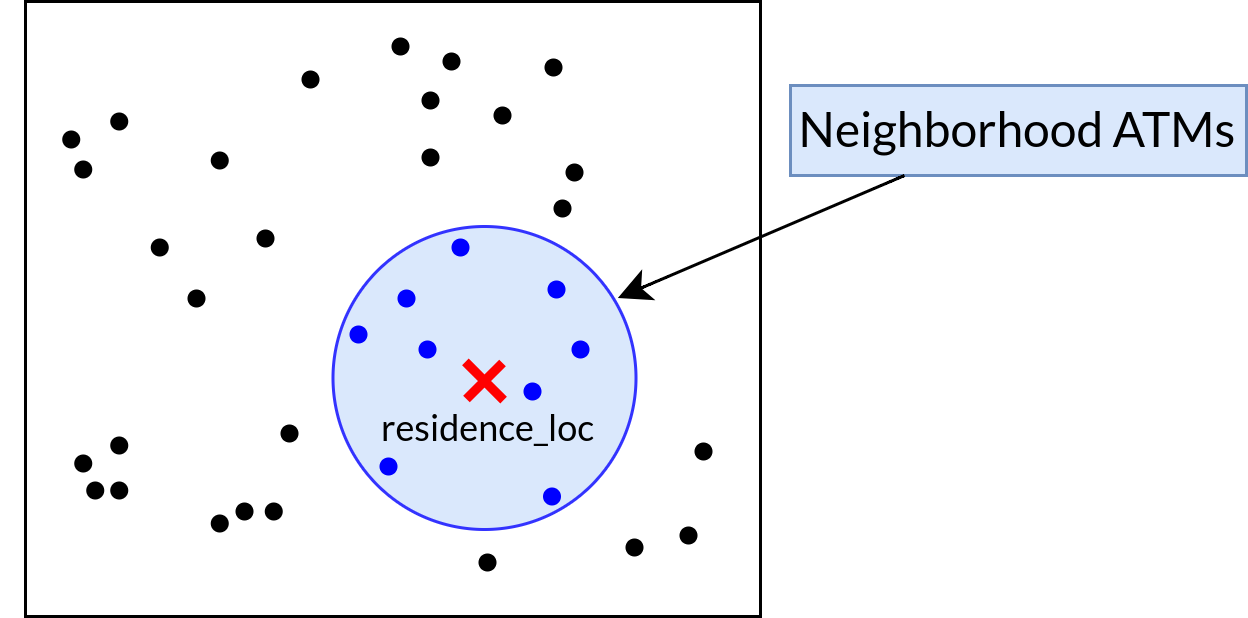
\includegraphics[scale=0.7]{figures/tx-generation-1-named.png}
\end{figure}
\end{frame}
\end{comment}
\begin{comment}
\begin{frame}{Experimental Design:: Regular transactions}

Set a minimum time distance $t_{min}$ between any two consecutive generated transactions of the client.%, based on the \emph{Neighborhood} subset.

    $$t_{min} = \frac{2 * \texttt{max\_distance}}{\texttt{max\_speed}}$$

    \begin{itemize}
        \item \textbf{max\_distance}: maximum distance from residence\_loc to an ATM $\in \ Neighborhood$ 
        {\tiny($\texttt{Neighborhood} = \{\texttt{ATM}\ | \texttt{dist(ATM, residence\_loc)} \leq \texttt{max\_distance}\}$).}
        
        \item \textbf{max\_speed}: maximum speed at which it is possible to travel (by any possible means of transport) between any pair of ATMs $\in \ \texttt{Neighborhood}$.
    \end{itemize}

\begin{figure}
    \centering
    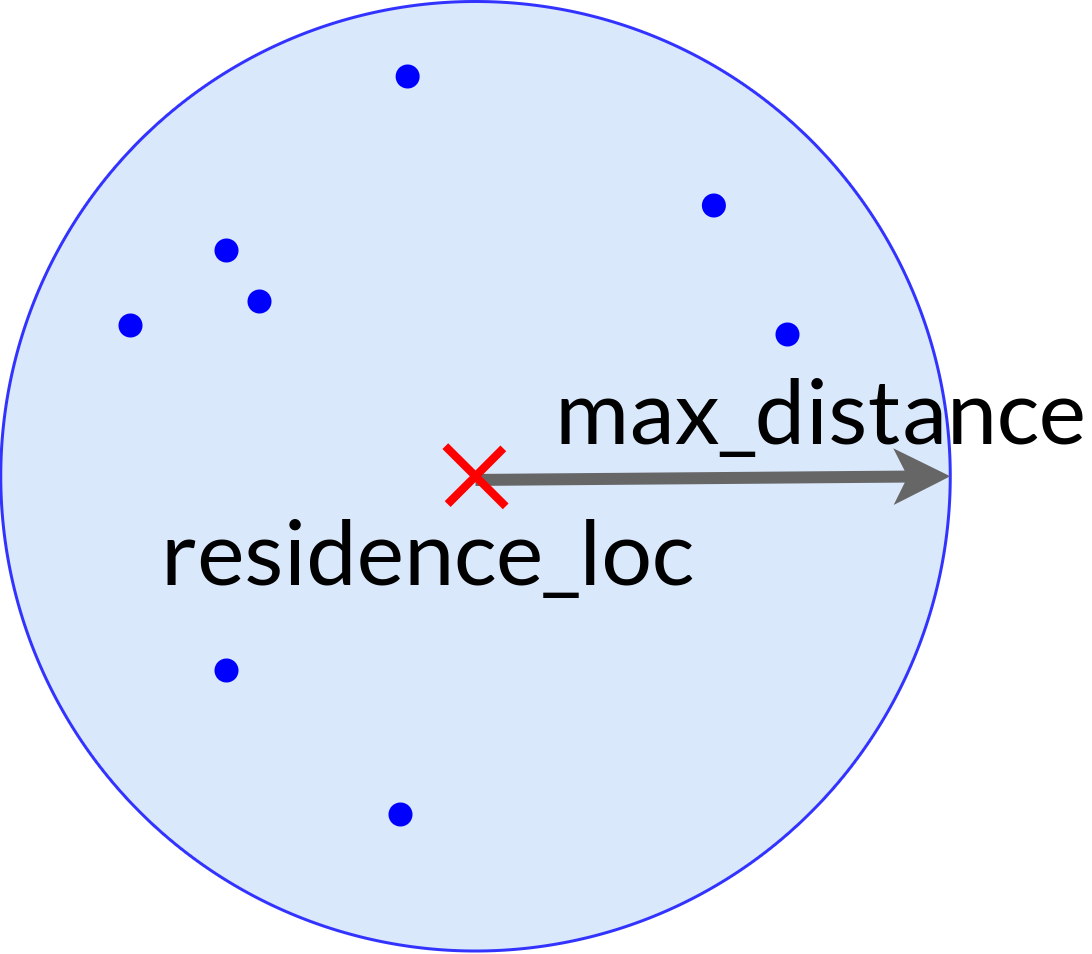
\includegraphics[scale=0.33]{figures/tx-generation-tmin.png}
\end{figure}
\end{frame}
\end{comment}

\begin{frame}{Experiments: Design of Experiments}
\begin{itemize}
    \item \textbf{E0: Evaluation in a real-world stress scenario}.
    \vspace{0.5em}
    \begin{itemize}
        \item[\textcolor{red}{$\rightarrow$}] Impractical simulation due to large time needed.
        \vspace{0.3em}
        \item[\textcolor{red}{$\rightarrow$}] Meaningless insights due to insufficient stress.
    \end{itemize}
    \vspace{1em}
    Therefore, two options were considered:
    \vspace{0.5em}
    \begin{itemize}
        \item[$(\text{i})$] Scaling of the transaction stream to smaller-sized time intervals streams.
        \vspace{0.3em}
        \item[$(\text{ii})$] Consider larger bank database system.
    \end{itemize}
    \vspace{2em}
    \item \underline{\textbf{E1: Evaluation in a high-load stress scenario}} - highest possible transaction stream frequency so to identify the system limits.
\end{itemize}
\end{frame}

\begin{frame}{Experiments: Considered Datasets}
\begin{itemize}
    \item Bank databases $g$:
    \vspace{1em}
    \begin{table}[H]
    \centering
    \begin{tabular}{|c|c|c|}
    \hline
    \textbf{Name} & \textbf{$|\text{Card}|$} & \textbf{$|\text{ATM}|$}  \\ \hline
    \smallG\  & 2,000      & 50 \\ \hline
    $\textbf{\textsf{GDB}}_{\textbf{\textsf{B}}}$ $\approx$ \textcolor{red}{Deutsche Bank Spain}  & 500,000      & 1,000     \\ \hline
    \end{tabular}
    \end{table}
\vspace{1em}
\item Synthetic streams $s(k, p)$, for each $g$:
\vspace{0.3em}
\begin{figure}
    \hspace*{-1.2cm}
    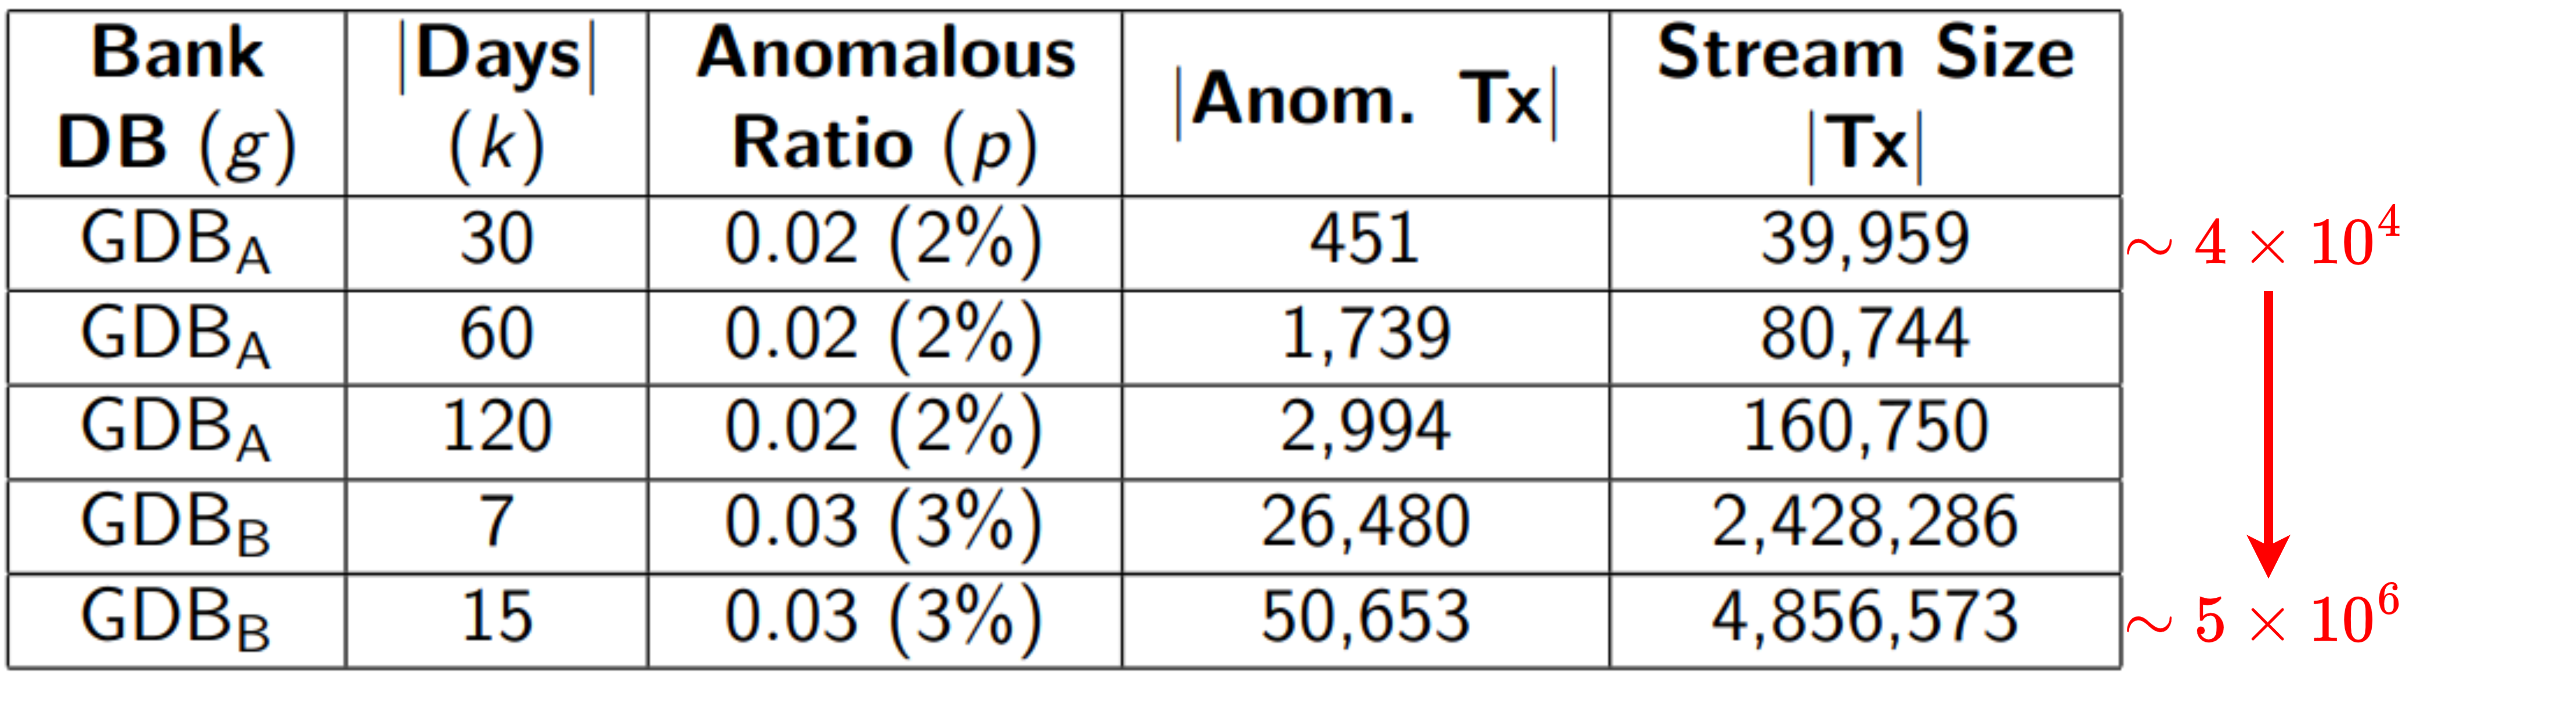
\includegraphics[scale=0.45]{figures/tableStreams.png}
\end{figure}
\end{itemize}
\end{frame}

\begin{comment}
\begin{table}[H]
    \small 
    \hspace*{-2cm}
    \begin{tabular}{|c|c|c|c|c|}
    \hline
    \begin{tabular}[c]{@{}c@{}}\textbf{Bank}\\ \textbf{DB} $(g)$ \end{tabular} &
    \begin{tabular}[c]{@{}c@{}}$|\textbf{Days}|$\\ $(k)$ \end{tabular}  & 
    \begin{tabular}[c]{@{}c@{}}\textbf{Anomalous}\\ \textbf{Ratio} ($p$)\end{tabular}  & \textbf{$|\text{Anom. Tx}|$} & 
    \begin{tabular}[c]{@{}c@{}}\textbf{Stream Size}\\ \textbf{$|\text{Tx}|$}\end{tabular} \\ \hline
    \smallG   & 30       & $0.02\ (2\%)$  & 451 & 39,959 \\ \hline
    \smallG    & 60       & $0.02\ (2\%)$ & 1,739 & 80,744 \\ \hline
    \smallG   & 120      & $0.02\ (2\%)$  & 2,994 & 160,750 \\ \hline
    \mediumG   & 7        & $0.03\ (3\%)$ & 26,480 & 2,428,286\\ \hline
    \mediumG  & 15       & $0.03\ (3\%)$ & 50,653 & 4,856,573\\ \hline
    \end{tabular}
\end{table}
\end{comment}


\begin{frame}{Experiments: E1 - Evaluation in a high-load stress scenario}
\textbf{Objectives}:
\begin{itemize}
    \item Comparison to sequential baseline.
    \item Analysis of the number of filters configuration.
    \item Analysis of the behavior and suitability of the \DPATM\ as a real-time engine.
\end{itemize}
\vspace{0.5em}
\textbf{Experimental variations}. $\Sigma= (g, s(k, p), f, c)$\\
with these combinations on:
\vspace{0.3em}
\begin{itemize}
    \item Number of filters $f$:
    \begin{itemize}
        \item $g = $ \smallG\ $f=1,2,5,10,20,40,100,200,500,1000,2000$.
        \item $g = $ \mediumG\ $f=1,5,10,100,250,500,1000,2000,5000,10000$.
    \end{itemize} 
    \item Number of cores: $c = 1, 2, 4, 8, 16$.
\end{itemize}
\vspace{0.7em}
$\Rightarrow$ {\small E.g. $\Sigma(\mathsf{GDB_A}, s(30, 0.02), f, c)$}
\end{frame}

\begin{frame}{Experiments: E1 - Evaluation in a high-load stress scenario}
\begin{itemize}
\item \textbf{Metrics:\\}
    \vspace{0.5em}
    As a real-time system, we evaluated the performance of the \DPATM\ in terms of:
    \vspace{0.5em}
    \begin{itemize}
        \item \textbf{Response Time} (\texttt{RT}) and \textbf{Mean Response Time} (\texttt{MRT}).
        \vspace{0.5em}
        \item \textbf{Execution Time} (\texttt{ET}).
        \vspace{0.5em}
        \item \textbf{Throughput} (\texttt{T}) (results emitted per second) and \textbf{Transactions per second} (\texttt{transactions/s}).
        \vspace{0.5em}
        \item \textbf{\texttt{dief@t}}: evaluation of the continuous emission of results. Introduced by Acosta, Vidal et al.\cite{AcostaVidal2017}.
        \vspace{0.5em}
        \item Number of \textbf{\texttt{checks}} and \textbf{\texttt{alerts}} (same number for each stream tested).
    \end{itemize}
\vspace{0.5em}
\item We consider all fraud pattern \textbf{\texttt{checks} as results} for experimental purposes. In a production version we will consider only \texttt{alerts} as results.

\end{itemize}

\end{frame}



